\begin{surferPage}[30 каспов]{Секстика Барта с $30$ каспами (точками возврата)\\{\normalfont\footnotesize(англ. „cusp“ — „заострение“)\par}}
После того, как Вольф Барт обнаружил секстику с максимально возможным количеством сингулярностей ($65$), двое из его аспирантов также установили своеобразные мировые рекорды для фигур более высоких степеней. Теперь он занимается поиском максимально возможного количества каспов (точек возврата) поверхности заданной степени.

   Конструкцию секстики Барта с $65$ сингулярностями типа
    $A_1^{+-}$ (т.е. двойной конус) можно адаптировать к каспам (всё же их количество составляет $30$): 
    \[P_6 - \alpha \cdot K^3=0,\]
  при этом $P_6$, как и в случае с другими секстиками Барта, являются плоскостями симметрии правильного икосаэдра, а $K$ – уравнение сферической поверхности:
    \vspace*{-0.4em} 
    \begin{center}
      \begin{tabular}{c@{\ }c@{\ }c@{\ }c}
        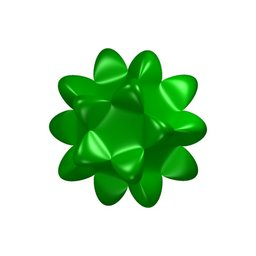
\includegraphics[height=1.2cm]{./../../common/images/barthsextic_30A2}
        &
        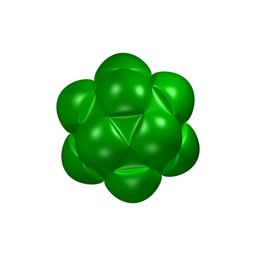
\includegraphics[height=1.2cm]{./../../common/images/barthsextic_30A2_3}
        &
        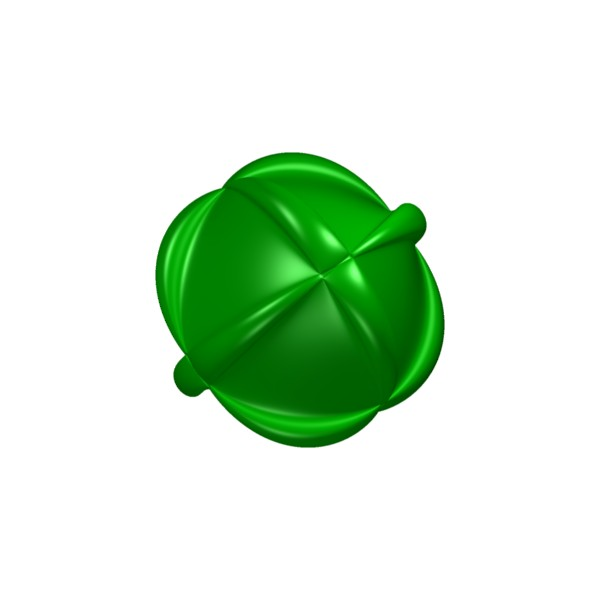
\includegraphics[height=1.2cm]{./../../common/images/barthsextic_30A2_5}
        &
        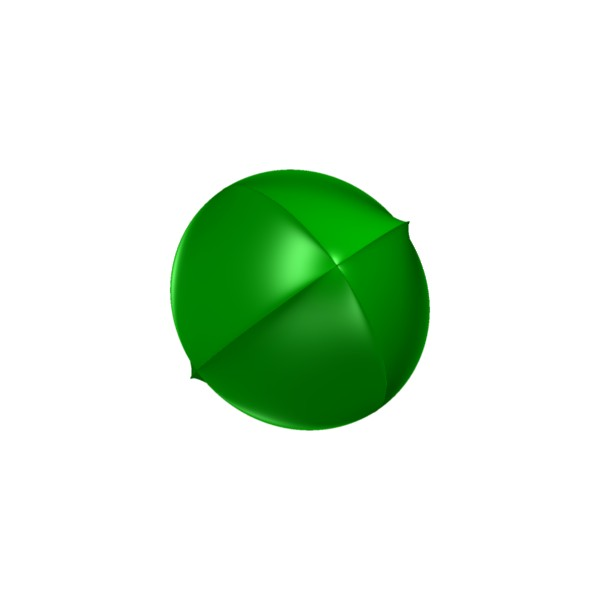
\includegraphics[height=1.2cm]{./../../common/images/barthsextic_30A2_6}
      \end{tabular}
    \end{center}    
    \vspace*{-0.3em}
Это и есть сегодняшний мировой рекорд: максимальное количество действительных каспов (точек возврата) на секстике, для комплексного пространства, оно достигает $36$.
\end{surferPage}
